\documentclass[12pt,a4paper]{report}

\usepackage{times}
\usepackage[german]{babel}
\usepackage{graphics}
\graphicspath{ {../img/} {../graph/img/} }
\usepackage{color}
\usepackage{ntheorem}
\theoremstyle{break}
\theorembodyfont{\normalfont}
\theoremprework{\bigskip\hrule\leavevmode}
\theorempostwork{\nopagebreak\hrule\leavevmode}
\newtheorem{exercise}{Aufgabe}[section]
\theoremstyle{plain}
\theoremprework{\bigskip\hrule\leavevmode}
\theorempostwork{\nopagebreak\hrule\leavevmode}
\newtheorem{proof}{Satz}[section]

\title{Minimale Spannb\"{a}ume}
\author{Gabriel Katz\\ Matthias Neeracher}

\begin{document}
\maketitle
\tableofcontents
\chapter{Einleitung}

\section{Wie kann hier gearbeitet werden?}

Dieser Text wird Sie mit einem wichtigen algorithmischen Problem
bekannt machen: dem Finden eines minimalen Spannbaums. Im n\"{a}chsten
Unterkapitel finden Sie eine Einf\"{u}hrung in das Thema, doch bevor
Sie loslegen, soll Ihnen hier noch kurz der Aufbau des Textes und die
Arbeitsweise damit erl\"{a}utert werden.

Die folgenden Kapitel sind zur selbstst\"{a}ndigen Bearbeitung
gedacht. Sie werden zuerst kurz Ihre Kenntnisse von ungerichteten
Graphen nochmals auffrischen, lernen dann die Theorie von B\"{a}umen
und gerichteten Graphen kennen, und lernen dann zwei verschiedene
Algorithmen, um einen \emph{minimalen Spannbaum} zu finden.
 
Wenn Sie einige dieser Begriffe jetzt noch nicht verstehen, macht das
nichts. Mitbringen sollten Sie aber die folgenden Kenntnisse:

\begin{itemize}
\item Sie wissen, was ein Algorithmus ist.
\item Sie kennen die Grundbegriffe ungerichteter Graphen (wir werden
  diese allerdings in Kapitel~\ref{graphs} kurz repetieren).
\end{itemize}

Zur behandelten Theorie finden Sie immer auch Aufgaben, anhand derer
Sie das Gelernte pr\"{u}fen k\"{o}nnen. Die L\"{o}sungen dieser Aufgaben stehen
jeweils im zweitletzten Unterkapitel f\"{u}r jedes Thema. Das letzte
Unterkapitel ist dann der Kapiteltest, den Sie bearbeiten und mit
Ihrer Lehrperson besprechen sollten.

\newpage
\section{Worum geht es hier?}

In den fr\"uhen 20er Jahren besch\"aftigte sich der tschechische
Mathematiker Otakar Bor\r{u}vka mit dem Problem, ein Gebiet (40
St\"{a}dte in S\"{u}d-M\"{a}hren) m\"{o}glichst effizient mit 
Elektrizit\"{a}t zu erschliessen.

\begin{figure}[h!]
\resizebox{!}{4cm}{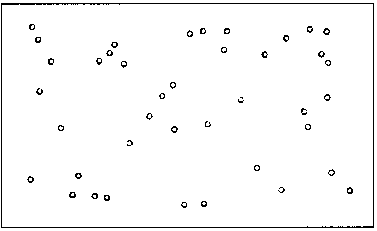
\includegraphics{BoruvkaPoints.pdf}}
\resizebox{!}{4cm}{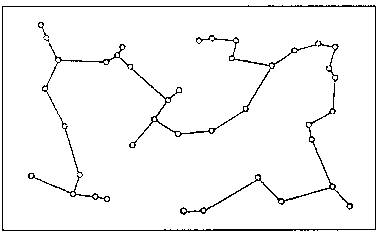
\includegraphics{BoruvkaTree.pdf}}
\caption{Elektrische Erschliessung von S\"{u}d-M\"{a}hren.\protect\footnotemark}
\end{figure}

\footnotetext{ 
Otakar  Bor\r{u}vka, \emph{O jist\'{e}m probl\'{e}mu minim\'{a}ln\'{i}m} (\"{U}ber ein
  gewisses Minimalisierungsproblem). \\
Zitiert aus: J. Ne\v{s}et\v{r}il,
  E. Milkov\'{a}, H. Ne\v{s}et\v{r}ilov\'{a}, \emph{Otakar Bor\r{u}vka
    on minimum spanning tree problem: translation of both the 1926
    papers, comments, history.}, Discrete Mathematics 233 (201)}
Sein Ansatz war, das Problem als Graphen abzubilden, in dem die
anzuschliessenden St\"{a}dte als Knoten, und die Distanzen zwischen ihnen
als Kanten repr\"{a}sentiert wurden. Das Elektrifizierungsproblem
besteht somit darin, alle Knoten so zu verbinden, dass die
Gesamtl\"{a}nge der Kanten so kurz wie m\"{o}glich bleibt. Eine solche
Verbindung wird \textbf{minimal aufspannender Baum} oder kurz
\textbf{minimaler Spannbaum} genannt.

Bor\r{u}vka's L\"{o}sung, die er 1926 publizierte, gilt als der erste
Algorithmus zur Konstruktion eines minimalen Spannbaums, und als einer
der ersten Optimierungs-Algorithmen. Weil sowohl
die Problemstellung als auch die verwendeten Algorithmen interessant
und einigermassen leicht verst\"{a}ndlich sind, werden wir uns jetzt diesem Problem widmen.

\chapter{Graphen}
\label{graphs}

\section{Rekapitulation: Was ist ein Graph?}

Ein \textbf{Graph} $G(V,E)$ besteht aus einer Menge von
\textbf{Knoten} $V$ und einer Menge von Kante $E$. Eine \textbf{Kante}
besteht aus einem Paar von Knoten, den \textbf{Endknoten} der
Kante. Wenn diese Paare geordnet sind, ist der Graph
\textbf{gerichtet}; die Kanten verbinden die Knoten nur in eine
Richtung. 

In diesem Text befassen wir uns aber nur mit
\textbf{ungerichteten} Graphen, in welchen die Knotenpaare ungeordnet
und somit die Knoten symmetrisch verbunden sind.  Des weiteren
beschr\"{a}nken wir uns auf \textbf{schlichte} Graphen, in denen keine
Kanten einen Knoten mit sich selbst verbinden, und zwischen zwei
Knoten nicht mehr als eine Kante existiert.

\begin{exercise}
Welche dieser vier Graphen sind gerichtet, welche ungerichtet? Welche
sind schlicht?

\scalebox{0.4}{\includegraphics{UngerichtetUnschlicht.pdf}}
\scalebox{0.4}{\includegraphics{Gerichtet.pdf}}
\scalebox{0.4}{\includegraphics{Ungerichtet.pdf}}
\scalebox{0.4}{\includegraphics{GerichtetUnschlicht.pdf}}
\end{exercise}

\section{Beschreibung von Graphen}
\label{Beschreibung}
\noindent Ein Graph $G(V,E)$ kann auf verschiedene Arten beschrieben werden:

\begin{description}
\item[Grafisch] indem die Knoten und Kanten aufgezeichnet werden:

\scalebox{0.5}{\includegraphics{Ungerichtet.pdf}}

gerade bei kleineren Graphen ist diese Darstellung f\"{u}r Menschen am
Einfachsten zu verstehen, aber sie ist z.B. f\"{u}r
Computerverarbeitung nicht besonders gut geeignet.
\item[Mengentheoretisch] indem die Knoten- und die Kantenmenge
  beschrieben werden:

\begin{displaymath}
V = \{\mathsf{A,B,C,D,E}\}\hspace{2cm}E = \{\mathsf{(A,B), (B,C),
  (C,D), (C,E), (B,E)}\}
\end{displaymath}

\item[\textnormal{als} Adjazenzmatrix] indem die Kanten als $n\times{n}$ Matrix $A(G)$
  dargestellt werden, wo der Eintrag $a_{ij}$ gleich $1$ ist, wenn eine Kante
  von Knoten $i$ nach Knoten $j$ existiert, und sonst gleich $0$.

\begin{displaymath}
A(G) = \left( 
\begin{array}{ccccc}
0 & 1 & 0 & 0 & 0 \\
1 & 0 & 1 & 0 & 1 \\
0 & 1 & 0 & 1 & 1 \\
0 & 0 & 1 & 0 & 0 \\
0 & 1 & 1 & 0 & 0 
\end{array}
\right)
\end{displaymath}

Wie zu beobachten ist, ist die Adjazenzmatrix bei einem ungerichteten
Graphen immer symmetrisch.
\end{description}

\begin{exercise}
\begin{itemize}
\item Zeichnen Sie einen ungerichteten Graphen $G(V,E)$ mit Knoten 
$V = \{\mathsf{A,B,C,D,E}\}$ und Kanten 
$E = \{\mathsf{(A, B), (A, D), (C, D), (A, E)}\}$.
\item Konstruieren sie die Adjazenzmatrix dieses Graphen.
\end{itemize}
\end{exercise}

\section{Zusammenh\"{a}ngende Graphen}

Wenn in einem Graphen $G(V,E)$ eine Folge von Knoten $v_0, v_1,
\ldots, v_n \in V$ existiert, die von Kanten $e_i = (v_i, v_i+1) \in
E$ verbunden werden, dann existiert ein \textbf{Weg} von $v_0$ nach
$v_n$. 

Falls ein Weg f\"{u}r \emph{jedes} Knotenpaar $v_0, v_n
\in V$ existiert, nennen wir den Graphen \textbf{zusammenh\"{a}ngend}.

Ein Weg $v_0\cdots{v_1}\cdots\ldots\cdots{v_0}$, der von einem Knoten
$v_0$ wieder auf diese selbst zur\"{u}ckf\"{u}hrt, heisst
\textbf{geschlossen}. Ein \textbf{zyklischer} Graph besteht aus einen
geschlossenen Weg, der alle Knoten und alle Kanten enth\"{a}lt.

\begin{exercise}
\textcolor{red}{Irgendwelche Ideen?}
\end{exercise}

\section{Untergraphen}

Ein Graph $U(W,F)$ ist ein \textbf{Untergraph} eines Graphen $G(V,E)$
wenn seine Knotenmenge $W$ eine Untermenge der Knotenmenge $V$ ist und
seine Kantenmenge $F$ eine Untermenge der Kantenmenge $E$.

\begin{exercise}
Welche der folgenden drei Graphen sind Untergraphen des Graphen in
Abschnitt~\ref{Beschreibung} ?

\scalebox{0.4}{\includegraphics{Sub1.pdf}}
\scalebox{0.4}{\includegraphics{Sub2.pdf}}
\scalebox{0.4}{\includegraphics{Sub3.pdf}}

\end{exercise}
\begin{exercise}
\textbf{FAKULTATIV} Wie viele Untergraphen $\mathcal{U}_n$ hat ein
\emph{vollst\"{a}ndiger} Graph 
\[ 
G(V = \{v_1, v_2, \ldots, v_n\}, E = \{(v_a, v_b) | v_a, v_b \in V,
v_a \neq v_b\}) ?
\] 
Finden Sie eine rekursive Definition $\mathcal{U}_n = f(\mathcal{U}_{n-1})$.
\end{exercise}

\newpage
\section{Gewichtete Graphen}
\label{gewichtet}

In vielen praktischen Anwendungen sind die Knoten und/oder Kanten
eines Graphen mit \textbf{Gewichten} versehen. Die Kantengewichte k\"{o}nnen
z.B. Distanz oder Flugkosten darstellen, die Knotengewichte
z.B. Hotelkosten.

\begin{exercise}
Der folgende Graph zeigt Flug- und Hotelkosten, sowie Reisedistanzen
f\"{u}r eine Reise.

\scalebox{0.5}{\includegraphics{Travel.pdf}}

\begin{itemize}
\item Was ist die \emph{k\"{u}rzeste} Route zwischen Z\"{u}rich und
    Sydney?
\item Was ist die \emph{billigste} Route?
\end{itemize}
\end{exercise}

 In der weiteren Diskussion werden wir hier nur noch an \textbf{Kantengewichteten} Graphen interessiert sein.

\section{L\"{o}sungen}

\textcolor{red}{To Be Completed}

\section{Kapiteltest}

\textcolor{red}{To Be Completed}

\chapter{B\"{a}ume}

\section{Was ist ein Baum?}

Als \textbf{Baum} bezeichnet man einen Graphen, der
\emph{zusammenh\"{a}ngend} ist und \emph{keinen geschlossenen Weg}
enth\"{a}lt. Eine Menge von B\"{a}umen, die keine gemeinsamen Knoten
haben, bezeichnet man (anschaulicherweise) als \textbf{Wald}.

\textcolor{red}{Aufgaben: Baeume identifizieren}

\begin{proof}
Ein Baum mit $n$ Knoten hat exakt $n-1$ Kanten.

\bigskip\noindent\textbf{Beweis:} Ein Baum mit $1$~Knoten kann keine Kanten haben.
In einem Baum mit $n$~Knoten sucht man sich einen beliebigen Knoten
aus, folgt einer beliebigen Kante, und beim n\"{a}chsten Knoten sucht
man sich eine andere Kante aus.
Weil der Baum ja keinen geschlossenen
Weg enth\"{a}lt, landet man irgendwann in einem Knoten, der von nur
$1$~Kante erreicht wird. 
Wenn man diesen Knoten und seine Kante aus
dem Baum entfernt, erh\"{a}lt man einen Baum mit $n-1$~Knoten, und
durch Induktion l\"{a}sst sich sehen, dass der Satz gilt.
\end{proof}

\section{Spannb\"{a}ume}

F\"ur jeden zusammenh\"{a}ngenden Graphen $G(V,E)$ kann man einen oder mehrere
\textbf{Spannb\"{a}ume} konstruieren, die aus \emph{allen Knoten} $V$ des
Graphen und einer \emph{Untermenge der Kanten} $E$ bestehen.

\textcolor{red}{Aufgaben: Alle aufspannenden Baeume fast vollstaendiger 4-Graph}

\section{Minimale Spannb\"{a}ume}

Wenn wir jetzt wieder an das in Kapitel~\ref{gewichtet}
eingef\"{u}hrten Konzept des \emph{kantengewichteten Graphen}
zur\"{u}ckdenken, k\"{o}nnen wir dieses auch auf B\"{a}ume
anwenden. Das \textbf{Gewicht} eines Baumes l\"{a}sst sich dann als
Summe der Kantengewichte des Baumes definieren.

\textcolor{red}{Aufgabe: Gewicht}

Somit k\"{o}nnen wir nun den zentralen Begriff dieses Textes
definieren: Ein Spannbaum $B$ eines Graphen $G$ ist ein
\textbf{minimaler Spannbaum} von $G$ wenn kein Spannbaum von $G$
existiert, dessen Gewicht kleiner als das Gewicht von $B$ ist.

Ein Graph kann ohne weiteres mehrere minimale Spannb\"{a}ume haben:
Wenn z.B. alle Kantengewichte identisch sind, sind \emph{alle}
Spannb\"{a}ume minimal!

\textcolor{red}{Aufgaben}

\section{L\"{o}sungen}
\textcolor{red}{To Be Completed}
\section{Kapiteltest}
\textcolor{red}{To Be Completed}

\chapter{Algorithmen}
\section{Der Algorithmus von Kruskal}
\textcolor{red}{To Be Completed}
\section{Der Algorithmus von Prim}
\textcolor{red}{To Be Completed}
\section{L\"{o}sungen}
\textcolor{red}{To Be Completed}
\section{Kapiteltest}
\textcolor{red}{To Be Completed}

\end{document}
